% Kartik Jain: portfolio and work record (long-form, public).
% Source of truth: resume/CAREER.md. Every claim here must trace back to it.
% Build:  npm run resume -- Kartik_Jain_Portfolio   ->  public/resume/Kartik_Jain_Portfolio.pdf
% Engine: tectonic (XeTeX). Body font XCharter; labels Source Sans Pro; code Source Code Pro.
% Section bodies live in parts/ so only this top-level file is compiled.

\documentclass[10pt,a4paper]{article}
\usepackage[fontsize=10.25pt]{scrextend}

% ---------------------------------------------------------------- page
\usepackage[
  a4paper,
  top=25mm, bottom=26mm, left=22mm, right=22mm,
  headheight=14pt, headsep=8mm, footskip=12mm,
]{geometry}

% ---------------------------------------------------------------- fonts
\usepackage{XCharter}   % loads fontspec under XeTeX
\setsansfont{SourceSansPro}[
  Extension=.otf, UprightFont=*-Regular, BoldFont=*-Semibold,
  ItalicFont=*-RegularIt, BoldItalicFont=*-SemiboldIt]
\setmonofont{SourceCodePro}[
  Extension=.otf, UprightFont=*-Regular, BoldFont=*-Semibold, Scale=0.84]
% Tracked caps for labels. LetterSpace above 6 breaks pdftotext word detection.
\newfontfamily\trackedfont{SourceSansPro}[
  Extension=.otf, UprightFont=*-Semibold, LetterSpace=6]
\newfontfamily\labelfont{SourceSansPro}[
  Extension=.otf, UprightFont=*-Semibold, BoldFont=*-Bold]

% ---------------------------------------------------------------- colour
\usepackage[table]{xcolor}
\definecolor{ink}{HTML}{1E1B17}
\definecolor{muted}{HTML}{6D655B}
\definecolor{hair}{HTML}{D8D0C2}
\definecolor{accent}{HTML}{A8492A}   % "Ember" accent from jkartik.in (light theme)
\definecolor{wash}{HTML}{F6F2EB}     % faint paper tint for a few panels

% ---------------------------------------------------------------- packages
\usepackage{microtype}
\usepackage{titlesec}
\usepackage{fancyhdr}
\usepackage{lastpage}
\usepackage{tabularx}
\usepackage{booktabs}
\usepackage{array}
\usepackage{enumitem}
\usepackage{calc}
\usepackage{tikz}
\usetikzlibrary{arrows.meta, positioning, fit, calc}
\usepackage[
  pdftitle={Kartik Jain - Portfolio and Work Record},
  pdfauthor={Kartik Jain},
  pdfsubject={Security and backend engineering: experience, security research, projects, leadership},
  pdfkeywords={Kartik Jain, security engineer, backend engineer, portfolio, Mumbai, NMIMS MPSTME},
  pdfcreator={Kartik Jain},
  colorlinks=true, linkcolor=ink, urlcolor=accent, citecolor=ink,
  bookmarksnumbered=false, pdfdisplaydoctitle=true,
]{hyperref}
\usepackage{bookmark}

% ---------------------------------------------------------------- text block
\setlength{\parindent}{0pt}
\setlength{\parskip}{4.8pt plus 1pt minus 1pt}
\linespread{1.07}
\frenchspacing
\widowpenalty=10000
\clubpenalty=10000
\emergencystretch=1.5em
\arrayrulecolor{hair}
\setlength{\arrayrulewidth}{0.4pt}

\setlist{nosep}
\setlist[itemize]{leftmargin=1.1em, itemsep=2.5pt, topsep=3pt, label={\color{muted}\raisebox{0.15ex}{\footnotesize\textbullet}}}

% ---------------------------------------------------------------- small macros
% Break only if the room is really not there. (needspace adds a stretchable, cheap break point
% that TeX prefers over a fuller page, which leaves half-empty pages. A negative remainder means the
% page builder is about to fire on its own, so forcing a break then would strand the leftover lines.)
\newcommand{\roomfor}[1]{\par\begingroup\dimen0=#1\relax\dimen2=\pagegoal\advance\dimen2 by -\pagetotal
  \ifdim\dimen2>0pt \ifdim\dimen0>\dimen2 \newpage\fi\fi\endgroup}
\newcommand{\tld}{{\sffamily\textasciitilde}}                     % approx. sign that sits on the baseline
\newcommand{\arr}{\,{\sffamily\color{muted}→}\,}                  % flow arrow in prose
\newcommand{\kicker}[1]{{\trackedfont\footnotesize\color{accent}\MakeUppercase{#1}}}
% \leavevmode first: a colour special at the top of a p-cell would shift the cell's baseline.
\newcommand{\lbl}[1]{\leavevmode{\trackedfont\scriptsize\color{muted}\MakeUppercase{#1}}}
\newcommand{\meta}[1]{{\sffamily\small\color{muted}#1}}
\newcommand{\runin}[1]{{\labelfont\small\color{ink}#1.}\enspace}
\newcommand{\code}[1]{{\ttfamily #1}}
\newcommand{\pref}[1]{p.\,\pageref{#1}}
\newcommand{\weblink}[2]{\href{#1}{#2}}

% Entry heading: title left, meta right, bookmarked.
\newcommand{\entry}[3][]{%
  \roomfor{7\baselineskip}\vspace{9pt}%
  \noindent\phantomsection\pdfbookmark[2]{#2}{bm:#2}%
  \ifx\relax#1\relax\else\label{#1}\fi
  {\fontsize{13.2}{16}\selectfont\bfseries #2}\hfill{\sffamily\small\color{muted}#3}\par
  \nopagebreak\vspace{1pt}}

% Smaller entry heading for compact lists.
\newcommand{\minientry}[3][]{%
  \roomfor{4\baselineskip}\vspace{5pt}%
  \noindent\phantomsection\pdfbookmark[3]{#2}{bm:mini:#2}%
  \ifx\relax#1\relax\else\label{#1}\fi
  {\bfseries #2}\hfill{\sffamily\footnotesize\color{muted}#3}\par\nopagebreak\vspace{0.5pt}}

% One-line summary under an entry heading.
\newcommand{\dek}[1]{\noindent{\itshape\color{ink}#1}\par\nopagebreak}

% Fact strip: label column + value column, hairlines above and below.
\newenvironment{facts}{%
  \par\vspace{3pt}\noindent\small
  \renewcommand{\arraystretch}{1.22}%
  \tabularx{\linewidth}{@{}>{\raggedright\arraybackslash}p{23mm}>{\raggedright\arraybackslash}X@{}}\toprule[0.4pt]}
  {\bottomrule[0.4pt]\endtabularx\par\vspace{4pt}}
\newcommand{\fact}[2]{\lbl{#1} & #2 \\}

% Sections: two-digit accent number, large serif title, hairline.
\renewcommand{\thesection}{\ifnum\value{section}<10 0\fi\arabic{section}}
\titleformat{\section}[display]
  {\normalfont\fontsize{21}{25}\selectfont\color{ink}}
  {{\trackedfont\small\color{accent}\thesection}}
  {5pt}
  {}
  [\vspace{3pt}{\color{hair}\titlerule[0.5pt]}]
\titlespacing*{\section}{0pt}{0pt}{9pt}
% Sections flow on, but never open in the last third of a page.
\newcommand{\sectionbreak}{\roomfor{0.33\textheight}\vspace{20pt}}

\titleformat{\subsection}[block]
  {\normalfont\labelfont\small\color{accent}}
  {}{0pt}{\MakeUppercase}
\titlespacing*{\subsection}{0pt}{14pt}{3pt}

% ---------------------------------------------------------------- running head / foot
\pagestyle{fancy}
\fancyhf{}
\renewcommand{\headrulewidth}{0pt}
\renewcommand{\footrulewidth}{0pt}
\fancyhead[L]{{\trackedfont\scriptsize\color{muted}KARTIK JAIN \,·\, PORTFOLIO AND WORK RECORD}}
\fancyhead[R]{{\sffamily\footnotesize\color{muted}\nouppercase{\rightmark}}}
\fancyfoot[L]{{\sffamily\footnotesize\color{muted}jkartik.in}}
\fancyfoot[R]{{\sffamily\footnotesize\color{muted}\thepage\ / \pageref*{LastPage}}}
\renewcommand{\sectionmark}[1]{\markright{#1}}
\renewcommand{\subsectionmark}[1]{}
\setcounter{secnumdepth}{1}
\fancypagestyle{cover}{%
  \fancyhf{}%
  \fancyfoot[L]{{\sffamily\footnotesize\color{muted}jkartik.in}}%
  \fancyfoot[R]{{\sffamily\footnotesize\color{muted}\thepage\ / \pageref*{LastPage}}}}

% ---------------------------------------------------------------- document
\begin{document}
\color{ink}

% ---------------------------------------------------------------- cover (page 1)
\thispagestyle{cover}
\pdfbookmark[1]{Kartik Jain}{bm:cover}

\vspace*{14mm}
\kicker{Portfolio and work record \,·\, October 2026}\par
\vspace{16pt}
{\fontsize{50}{54}\selectfont Kartik Jain}\par
\vspace{9pt}
{\fontsize{20}{24}\selectfont\itshape Security \& Backend Engineer}\par
\vspace{18pt}
{\sffamily\small\color{muted}%
Mumbai \enspace·\enspace
\href{mailto:career@jkartik.in}{career@jkartik.in} \enspace·\enspace
\href{https://jkartik.in}{jkartik.in}\par
\vspace{1pt}
\href{https://github.com/KartikJain14}{github.com/KartikJain14} \enspace·\enspace
\href{https://www.linkedin.com/in/kartikjain1410}{linkedin.com/in/kartikjain1410}\par}
\vspace{14pt}
{\color{hair}\rule{\linewidth}{0.5pt}}
\vspace{8pt}

This document is the long-form record behind the
\href{https://jkartik.in/Kartik_Resume.pdf}{one-page résumé}. Each role and project is described
with its context, the approach taken and the outcome. Ownership is stated plainly: solo, lead,
co-lead, maintainer or contributor.

\vfill

\subsection*{Contents}
\vspace{2pt}
\newcommand{\tocrow}[3]{\noindent\makebox[8mm][l]{\sffamily\footnotesize\color{accent}#1}\hyperref[#3]{#2}\hfill{\sffamily\footnotesize\color{muted}\pageref*{#3}}\par\vspace{2.5pt}}
\noindent\begin{minipage}[t]{0.56\linewidth}
\setlength{\parskip}{0pt}
\tocrow{01}{Experience}{sec:exp}
\tocrow{02}{Security research}{sec:research}
\tocrow{03}{Selected projects}{sec:projects}
\tocrow{04}{Leadership and community}{sec:lead}
\tocrow{05}{Achievements}{sec:awards}
\tocrow{06}{Skills, with evidence}{sec:skills}
\tocrow{07}{Education}{sec:edu}
\tocrow{08}{Links}{sec:links}
\end{minipage}\par
\vspace{6mm}

\clearpage

% ---------------------------------------------------------------- at a glance (page 2)
\section*{At a glance}\label{sec:glance}
\markright{At a glance}
\pdfbookmark[1]{At a glance}{bm:glance}

Kartik Jain is a security and backend engineer in Mumbai and a B.Tech Information Technology
student at NMIMS MPSTME (2024--2028, CGPA 8.34/10.0). As a Software Engineer Intern at VisionRise
Technosoft, Kartik built a white-label learning platform end to end and shipped it as two Google
Play apps. As a Security Engineer Intern at R.U.D.R.A Cybersecurity, a Mumbai VAPT firm, Kartik
found two high-severity flaws in a banking client's portal and automated attack-surface
monitoring. Alongside both: a \$1,500 bug bounty from Meta, vulnerability reports to Microsoft and
(through CERT-In) the Mumbai Police, freelance backend and incident-response work, and the technical
side of several college organisations, most recently as Chairperson of ACM MPSTME.

\subsection*{Strongest areas}
\vspace{2pt}
{\small
\renewcommand{\arraystretch}{1.0}%
\noindent\begin{tabularx}{\linewidth}{@{}>{\raggedright\arraybackslash}X@{\hspace{7mm}}>{\raggedright\arraybackslash}X@{\hspace{7mm}}>{\raggedright\arraybackslash}X@{}}
{\labelfont Application security}\par\vspace{2pt}
Web-application penetration testing, manual code review and coordinated disclosure, with
findings reported to Meta, Microsoft (MSRC) and CERT-In. LLM red teaming: 1st place on the global
leaderboard of chat.win's AI Jailbreakathon.
&
{\labelfont Backend engineering}\par\vspace{2pt}
APIs in TypeScript/Node.js and Python on PostgreSQL, with the decisions that matter enforced on
the server: authentication, role-based access, signed payment webhooks, encrypted media delivery
and race-free check-ins.
&
{\labelfont Running production}\par\vspace{2pt}
Hardened Ubuntu servers, Docker and Coolify CI/CD, automated backups to cloud storage, self-hosted
mail with SPF, DKIM and DMARC, and incident response when a client platform was hit by ransomware.
\end{tabularx}}

\subsection*{In numbers}
\vspace{3pt}
\newcommand{\stat}[2]{%
  \leavevmode{\fontsize{19}{22}\selectfont\color{accent}#1}\par\vspace{1.5pt}%
  {\footnotesize\color{muted}#2}\par\vspace{13pt}}
{\renewcommand{\arraystretch}{1.0}%
\noindent\begin{tabularx}{\linewidth}{@{}>{\raggedright\arraybackslash}X@{\hspace{7mm}}>{\raggedright\arraybackslash}X@{\hspace{7mm}}>{\raggedright\arraybackslash}X@{}}
\stat{\$1,500}{bug bounty awarded by Meta for a privilege escalation in WhatsApp}
& \stat{276}{REST routes across 20 modules in the LMS backend built at VisionRise}
& \stat{\tld4,000}{students on the official Railway Concession system Kartik maintains} \\
\stat{16,000+}{users on a client platform Kartik hardened and brought back after ransomware}
& \stat{\tld\$20,000/yr}{saved by automating attack-surface monitoring at R.U.D.R.A}
& \stat{600+ \,/\, 500+}{delegates served by the Delego and conc-qr event backends} \\
\stat{1,100+}{hackathon participants onboarded automatically by a Discord bot}
& \stat{\tld500}{learners in Programming For Everyone, a record, as ACM Chairperson}
& \stat{1st}{place on the global leaderboard of chat.win's AI Jailbreakathon} \\
\end{tabularx}}

\subsection*{Looking for}
Internships in security engineering or backend development, and freelance engagements in
web-application security testing and backend development. Graduating in April 2028.
Contact: \mbox{\href{mailto:career@jkartik.in}{career@jkartik.in}}.

\clearpage

% ---------------------------------------------------------------- experience
\section{Experience}\label{sec:exp}

% ............................................................ VisionRise
\entry[exp:visionrise]{VisionRise Technosoft Pvt.\ Ltd.}{Apr 2026 -- Oct 2026 · Mumbai}
\dek{Software Engineer Intern. Built the company's white-label learning platform and ran its production server.}

\begin{facts}
\fact{Company}{Edtech and software company behind the Rise Academy / Rise Institute and eGuru brands
  (\href{https://risetechnosoft.com}{risetechnosoft.com})}
\fact{Ownership}{Created and wrote nearly all of the LMS v2 codebase and the eGuru fork; contributed to
  the earlier, team-built LMS v1}
\fact{Stack}{TypeScript, Node.js, Express, PostgreSQL, Drizzle ORM, Zod, JWT, React Native, Expo,
  FFmpeg, Google Cloud Storage, Gemini, Zoom, Docker, Coolify, Ubuntu 24.04 LTS}
\fact{Live}{\href{https://play.google.com/store/apps/details?id=tech.riseinstitute.app}{Rise Academy}
  and \href{https://play.google.com/store/apps/details?id=app.eguru.lms}{eGuru} on Google Play
  \,·\, \href{https://riseinstitute.tech}{riseinstitute.tech} \,·\, \href{https://eguru.app}{eguru.app}}
\end{facts}

\runin{Context} LMS v2 is a white-label learning platform: one backend and one app codebase that
ship under more than one brand, covering courses, live classes, assessments and paid video for
students on Android, iOS and the web. Kartik built it from the database schema to the store
listing, then forked it into eGuru, a second branded app.

\runin{Backend architecture} A Node.js/Express API in TypeScript (\tld40,000 lines), organised into
20 domain modules that together expose 276 REST routes: admin, AI, analytics, assignments, audit,
auth, calendar, certificates, courses, enrollments, lessons, live classes, media, modules,
notifications, payments, quizzes, reports, settings and users. Inputs are validated with Zod at the
boundary, data lives in PostgreSQL with schema changes tracked as Drizzle migrations, and the
repository carries 25 test files.

\runin{One app, three platforms} The client is a single React Native/Expo codebase (\tld45,000
lines) that builds for Android, iOS and the web, with push notifications and over-the-air updates
through Expo, so fixes reach installed apps without waiting on a store release.

\runin{Protecting paid content} Paid video is the asset most worth protecting. Uploads go through an
FFmpeg transcoding pipeline that produces AES-128-encrypted HLS. Playback needs a per-session token
that the API validates on every segment request, and media is fetched through short-lived signed
Google Cloud Storage URLs, so a copied link expires quickly and does not work outside the session
that requested it. PDFs stream inside the app with no download surface, and course certificates
can be verified through a SHA-256 hash.

\begin{center}
\vspace{2pt}
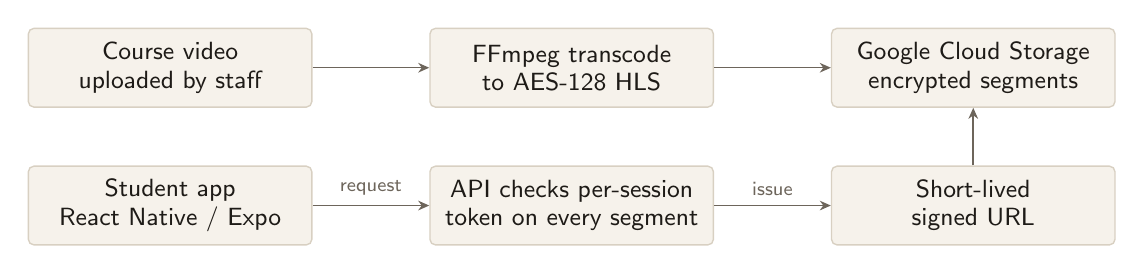
\begin{tikzpicture}[
  font=\sffamily\footnotesize,
  box/.style={draw=hair, line width=0.5pt, rounded corners=2pt, fill=wash, text=ink,
              align=center, inner xsep=5pt, inner ysep=4pt, minimum width=36mm, minimum height=10mm},
  arrow/.style={-{Stealth[length=4pt,width=3.5pt]}, draw=muted, line width=0.55pt},
  tag/.style={font=\sffamily\scriptsize, text=muted}]
  \node[box] (up)  at (0,0)      {Course video\\uploaded by staff};
  \node[box] (ff)  at (5.1,0)    {FFmpeg transcode\\to AES-128 HLS};
  \node[box] (gcs) at (10.2,0)   {Google Cloud Storage\\encrypted segments};
  \node[box] (app) at (0,-1.75)  {Student app\\React Native / Expo};
  \node[box] (api) at (5.1,-1.75){API checks per-session\\token on every segment};
  \node[box] (url) at (10.2,-1.75){Short-lived\\signed URL};
  \draw[arrow] (up) -- (ff);
  \draw[arrow] (ff) -- (gcs);
  \draw[arrow] (app) -- node[tag, above]{request} (api);
  \draw[arrow] (api) -- node[tag, above]{issue} (url);
  \draw[arrow] (url) -- (gcs);
\end{tikzpicture}\par
\vspace{3pt}
{\footnotesize\itshape\color{muted}Paid-video path: content is encrypted when it is transcoded and is reachable only with a session token and an expiring URL.}
\end{center}

\runin{Authentication and access} Students sign in with Google or with a PIN tied to a phone number
verified over WhatsApp. Sessions use JWT access and refresh tokens, role-based access separates
admins, instructors and students, and admin actions are written to an audit log.

\runin{Features and integrations} Kartik built Live Classes v1 on Zoom: classes are orchestrated from
the platform, Zoom's webhooks are signature-verified before they are trusted, attendance and
recordings are captured, and Gemini then generates a quiz from the class content. Around this core
Kartik shipped courses, quizzes and assignments, UPI payment verification, push and email
notifications, and bulk enrollment.

\runin{Production server} Kartik provisioned and hardened the company's primary production server on
Ubuntu 24.04 LTS with a standard baseline: SSH key-only access, a firewall, unattended security
upgrades and fail2ban. The apps and PostgreSQL run behind Coolify, which handles CI/CD and
deployments; container and application logs are collected through Coolify and Docker; and automated
backups go to Google Cloud Storage.

\runin{IT administration} Kartik administered the company's GitHub organisation (15 repositories,
about 5--10 members) and its Google Workspace directory of 35+ accounts, covering accounts, access
and permissions.

\runin{Other work} Contributed to the earlier, team-built LMS v1: CI/CD, timezone-safe class
scheduling with the PostgreSQL session pinned to IST, course-invite and access-request flows, and
Zoom fixes. Built a government procurement-management prototype (FastAPI and React) for a client
demo, and the eguru.app marketing site as a Next.js static export.

\runin{Outcome} Two apps live on Google Play, Rise Academy and eGuru, built from one codebase and one
backend, and deployed through a pipeline onto a server that Kartik set up and maintained.

% ............................................................ R.U.D.R.A
\entry[exp:rudra]{R.U.D.R.A Cybersecurity Pvt.\ Ltd.}{May 2025 -- Jul 2025 · Mumbai}
\dek{Security Engineer Intern for three months at a Mumbai-based VAPT and offensive-security firm: client testing, internal tooling and purple-team exercises, using BBOT, Semgrep, Neo4j, Nuclei and Sliver C2.}

\runin{Attack-surface monitoring} Kartik automated recurring external attack-surface monitoring with
BBOT, cutting manual reconnaissance and saving \tld\$20,000 a year.

\runin{Static analysis at scale} Kartik single-handedly built a custom Semgrep (SAST) module with
Neo4j-based graph visualisation, for analysing large codebases.

\runin{Banking client} Manual code review of a banking client's web portal found two high-severity
vulnerabilities: a local file inclusion, and broken access control that exposed restricted
functionality to unauthorised users. Both were reported to the client, and Kartik then automated
their detection with custom Nuclei templates.

\runin{Purple teaming} Deployed and operated the Sliver C2 framework for purple-team exercises that
emulated real-world intrusions.

\runin{Outcome} Two high-severity findings for a client, a recurring recon task automated with a
\tld\$20,000-a-year saving, and an in-house SAST module.

% ............................................................ Freelance
\entry[exp:freelance]{Freelance}{May 2025 -- Oct 2026}
\dek{Self-employed Backend \& Security Engineer. Two separate engagements, not continuous; clients are not named.}

\minientry{Incident response and hardening}{May -- Jun 2025 · about one month}
A freelance client ran a web platform with 16,000+ users. Kartik hardened its server
infrastructure, and when the platform was hit by ransomware, led the incident response: contained
the attack and restored service through rapid backup and recovery.

\minientry[proj:sports]{sports-live: tournament auction and scoring platform}{Aug 2026 -- Oct 2026}
Built for a client and used at ELEV8, a pickleball tournament in which \tld200 players were
auctioned into 8 teams. The platform covers player registration and verification, a purse-based
live player auction with a board for the projector, fixtures, live scoring and standings. Venue
Wi-Fi is unreliable, so writes go into an offline queue in IndexedDB and are sent when the
connection returns.

\begin{facts}
\fact{Ownership}{Solo}
\fact{Stack}{Next.js 16, Supabase (PostgreSQL with row-level security, Realtime, Storage),
  server-side image processing, IndexedDB, Vitest}
\end{facts}

% ---------------------------------------------------------------- security research
\section{Security research}\label{sec:research}

Kartik reports vulnerabilities to the affected organisation or through its disclosure program, and
the technical detail below goes no further than what is published at
\href{https://jkartik.in/research/}{jkartik.in/research}. The work starts by hand, with manual code
review, Burp Suite and Nmap; what is learned is then automated with Nuclei, Semgrep and BBOT.

\vspace{2pt}
{\small
\renewcommand{\arraystretch}{1.3}%
\noindent\begin{tabularx}{\linewidth}{@{}>{\raggedright\arraybackslash}p{27mm}>{\raggedright\arraybackslash}X>{\raggedright\arraybackslash}p{41mm}@{}}
\toprule[0.4pt]
\lbl{Organisation} & \lbl{Finding} & \lbl{Channel and status} \\
\midrule[0.4pt]
WhatsApp (Meta) & Privilege-escalation vulnerability in WhatsApp. & Meta bug bounty program; \$1,500 bounty awarded (2022) \\
Microsoft & Access-control and information-disclosure issues in Intune, Entra/Azure and the Exchange
  Admin Center. Organisation member data was served before the authorization check completed, a
  time-of-check/time-of-use gap spanning Intune, Entra and Azure. Standard users could bypass
  ``restricted'' policies through the Exchange admin portal to edit directory name fields and join
  closed groups. & Reported to the Microsoft Security Response Center (MSRC) \\
Mumbai Police & Stored cross-site scripting on the official website. & Disclosed responsibly, in coordination with CERT-In \\
The Souled Store & Exposed staging infrastructure that could have allowed a full system compromise. & Reported \\
Belgian Waffle Co. & Source-code and credential leak that opened the door to a potential CRM takeover. & Reported \\
Banking client & Local file inclusion and broken access control, both high severity, found through
  manual code review; detection then automated with custom Nuclei templates (\pref{exp:rudra}). & Reported to the client during a R.U.D.R.A engagement \\
\bottomrule[0.4pt]
\end{tabularx}}

\subsection{Defensive work}

\minientry{Ransomware response and infrastructure hardening}{Freelance · May -- Jun 2025}
Hardened the server infrastructure of a web platform with 16,000+ users and, when ransomware hit
it, led the response that contained the attack and restored service through rapid backup and
recovery (\pref{exp:freelance}).

\subsection{Adversarial AI}

\begin{itemize}
  \item \textbf{1st place, global leaderboard}, AI Jailbreakathon by chat.win: an LLM prompt
        attack-and-defence contest, won with the fewest tokens (\$250 prize).
  \item \textbf{Fool The LLM}: built and ran a prompt-injection contest platform (\pref{proj:ftl}).
  \item \textbf{CSAW LLM Attack Challenge (LLMAC) '25}, NYU: participated.
  \item \textbf{Writing}: \href{https://jkartik.in/blog/where-llm-guardrails-break/}{``Where LLM
        guardrails break''}, a field report from the contest on what cracks guardrail prompts and
        how to design systems that do not depend on them.
\end{itemize}

% ---------------------------------------------------------------- selected projects
\section{Selected projects}\label{sec:projects}

Case studies first, then shorter entries. Ownership uses five fixed words: \emph{solo} (all
Kartik's work), \emph{lead} (majority author), \emph{co-lead} (a major share), \emph{maintainer}
(took over an existing system) and \emph{contributor} (a minority share). The one team project
says \emph{team of 3} instead. Source links appear where the repository is public.

% ............................................................ GhostShare
\entry[proj:ghostshare]{GhostShare}{Solo · 2026}
\dek{End-to-end-encrypted, ephemeral, real-time sharing: anonymous rooms, no accounts, and a server that only ever sees ciphertext.}

\begin{facts}
\fact{Stack}{TypeScript (strict), Next.js 15, React 19, Fastify 5, Socket.IO 4 with the Redis adapter,
  PostgreSQL 16 and Drizzle, BullMQ, Redis 7, Cloudflare R2, Web Crypto AES-256-GCM, Argon2id
  (hash-wasm), pnpm and Turborepo, Docker Compose behind Coolify, Pino, Sentry}
\fact{Links}{Live at \href{https://share.jkartik.in}{share.jkartik.in} \,·\, write-up:
  \href{https://jkartik.in/blog/zero-knowledge-sharing/}{``The server can't read this''} \,·\,
  \href{https://jkartik.in/projects/ghostshare/}{project page} \,·\, source is private}
\end{facts}

\runin{Problem} Most ``private'' sharing tools still hold plaintext and promise not to read it.
GhostShare is designed so that the server cannot.

\runin{Threat model} The design assumes the server is hostile: the database leaks, object storage
is public, and the operator reads the logs. Each room's secret lives in the URL fragment, which
browsers do not send to the server. The browser derives an AES-256 key from that secret with
Argon2id, a memory-hard function that makes offline guessing of a weak secret expensive, and seals
every note and file with AES-256-GCM, whose authentication tag also exposes tampering by a hostile
server.

\begin{center}
\vspace{2pt}
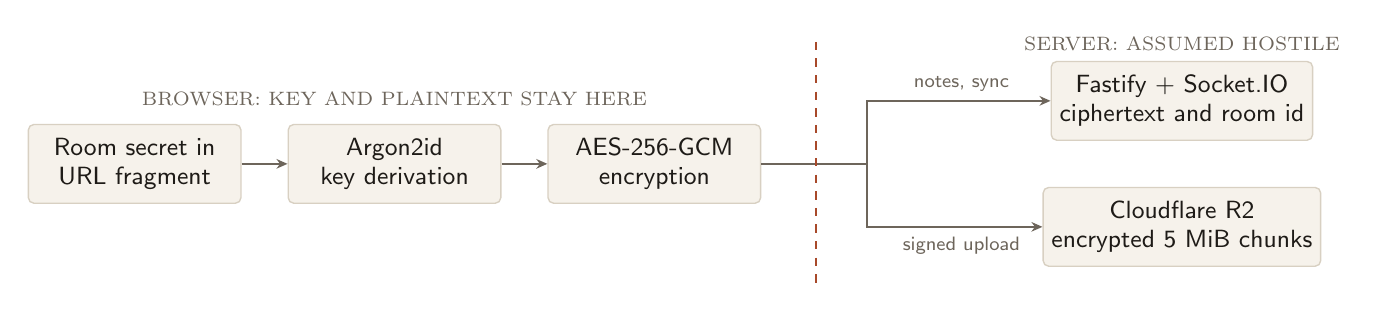
\begin{tikzpicture}[
  font=\sffamily\footnotesize,
  box/.style={draw=hair, line width=0.5pt, rounded corners=2pt, fill=wash, text=ink,
              align=center, inner xsep=3pt, inner ysep=4pt, minimum width=27mm, minimum height=10mm},
  arrow/.style={-{Stealth[length=4pt,width=3.5pt]}, draw=muted, line width=0.55pt},
  tag/.style={font=\sffamily\scriptsize, text=muted},
  zone/.style={font=\trackedfont\scriptsize, text=muted}]
  \node[box] (sec) at (0,0)   {Room secret in\\URL fragment};
  \node[box] (kdf) at (3.3,0) {Argon2id\\key derivation};
  \node[box] (enc) at (6.6,0) {AES-256-GCM\\encryption};
  \node[box, minimum width=31mm] (api) at (13.3,0.8)  {Fastify + Socket.IO\\ciphertext and room id};
  \node[box, minimum width=31mm] (r2)  at (13.3,-0.8) {Cloudflare R2\\encrypted 5 MiB chunks};
  \draw[arrow] (sec) -- (kdf);
  \draw[arrow] (kdf) -- (enc);
  \draw[arrow] (enc.east) -- (9.3,0) |- (api.west);
  \draw[arrow] (enc.east) -- (9.3,0) |- (r2.west);
  \node[tag, above] at (10.5,0.8) {notes, sync};
  \node[tag, below] at (10.5,-0.8) {signed upload};
  \draw[accent, dashed, line width=0.7pt] (8.65,1.55) -- (8.65,-1.55);
  \node[zone, anchor=south] at (3.3,0.62) {BROWSER: KEY AND PLAINTEXT STAY HERE};
  \node[zone, anchor=south] at (13.3,1.32) {SERVER: ASSUMED HOSTILE};
\end{tikzpicture}\par
\vspace{3pt}
{\footnotesize\itshape\color{muted}Encryption happens before anything reaches the network; the dashed line is the trust boundary.}
\end{center}

\runin{Large files} Files are split into 5 MiB chunks, encrypted in the browser and uploaded straight
to Cloudflare R2 with four parallel uploads, exponential-backoff retry and resume. The app server
hands out short-lived signed upload URLs and never touches the bytes.

\runin{Real time and expiry} Collaboration runs over Socket.IO with a Redis adapter, so it scales
horizontally while relaying only ciphertext. Edits made offline queue in IndexedDB and drain on
reconnect. Every room has a lifetime chosen at creation (1 day, 3 days, 1 week or 1 month), and an
hourly job purges expired rooms and orphaned storage. Helmet and rate limiting guard the API, and
backup and restore scripts cover the data that does persist.

\runin{Limits, stated in the write-up} Metadata such as timing and blob sizes stays visible to the
server, the client code that is served must be trusted, and a room keeps one key for its lifetime;
per-room key rotation is the planned next step.

% ............................................................ NeuroTechh (MAL 4)
\entry[proj:neurotechh]{NeuroTechh: clinic appointment platform}{Team of 3 · Nov 2026}
\dek{The first-prize entry at the MAL 4 hackathon: an architecture and prototype in which patients request appointment slots and clinics confirm or decline them.}

\begin{facts}
\fact{Event}{MAL 4 (Mobile Architecture Lab), Paytm, Mumbai, 1 November 2026. First prize, against working
  professionals and students.}
\fact{Stack}{React Native, Expo, Express, TypeScript, PostgreSQL, Redis, Measure SDK, Docker Compose}
\fact{Links}{Source and design documents:
  \href{https://github.com/KartikJain14/mal-hackathon}{github.com/KartikJain14/mal-hackathon} \,·\, write-up:
  \href{https://jkartik.in/blog/mal4-hackathon-where-code-was-optional/}{``We won a hackathon where the code was optional''}}
\end{facts}

\runin{What was judged} Architecture was 60\% of the score and code was optional. The team of three
submitted a one-page problem brief, a full platform design, an HLD, an LLD, 19 Architecture Decision
Records and three walkthroughs: the core path, failures and a new requirement. The rule the design
protects is that a confirmed slot belongs to exactly one patient and that a cancellation reopens the
slot consistently.

\runin{Key decisions} One modular API rather than the nine microservices first proposed. Postgres row
locks and a partial unique index rather than Redis locks. A transactional outbox rather than Kafka.
Pending requests hold no slot, so the race happens when a clinic confirms rather than when a patient
asks. Idempotency keys are created on the phone.

\runin{Prototype} Built for extra credit: patient, hospital and doctor flows, QR check-in, family
profiles and record uploads. Integration tests cover booking and workflows. The booking rule was
checked with 2, 50 and 200 concurrent confirms on one slot, and exactly one was confirmed each time.

\runin{Limits, stated in the repository} This is a hackathon design and prototype, not a deployed
service. The prototype writes outbox rows in the same transaction as each booking change, but the
worker that would deliver them exists only in the design. The repository's
\href{https://github.com/KartikJain14/mal-hackathon/blob/main/docs/architecture/as-built.md}{as-built
document} records what the code does and where it differs from the design.

% ............................................................ Railway Concession
\entry[proj:concession]{Railway Concession}{Maintainer · Jul 2026 -- present}
\dek{MPSTME's official online railway-concession system: student submissions, collection-slot booking and tools for the college office.}

\begin{facts}
\fact{Ownership}{The original 2025 version was built by the NeuroTechh team. Kartik took it over in
  July 2026 and now maintains it solo, working with the college administration as its rules change.}
\fact{Scale}{Used by \tld4,000 students}
\fact{Stack}{Next.js, PostgreSQL, Drizzle ORM, Nodemailer}
\fact{Links}{Live at \href{https://concession.mpst.me}{concession.mpst.me} \,·\, write-up:
  \href{https://jkartik.in/blog/when-a-form-becomes-infrastructure/}{``When a form becomes infrastructure''}}
\end{facts}

\runin{Data layer} Migrated the system to PostgreSQL with Drizzle ORM.

\runin{Booking rules on the server} A collection date is not accepted just because the browser's date
picker allowed it. One shared module validates every date against the lead time, weekends,
holidays, the configured end date and a rolling window of open dates, computed in Indian Standard
Time whatever the server's own timezone. The client asks the server for the current window only to
guide the student; the submission endpoint validates again before writing. The window slides forward
on its own, so opening a new day needs no deployment.

\runin{Tools for the office} Search by SAP ID with the student's full profile and submission history;
mark a form collected for any date; block SAP IDs; manage holidays; tune the booking window; and
export to Excel. Students get confirmation emails, and the office gets an automated daily
collection-report email. Kartik also patched vulnerable dependencies and improved SEO.

\runin{Outcome} A process that \tld4,000 students depend on, with rules the office can change from a
settings panel rather than waiting on a code change.

% ............................................................ Event & payment backends
\entry[proj:events]{Event and payment backends}{2024 -- 2026}
\dek{Four backends for NMIMS student events, each with one decision that has to be right: whether money changed hands, or whether a badge was already used.}

{\small
\renewcommand{\arraystretch}{1.25}%
\noindent\begin{tabularx}{\linewidth}{@{}>{\raggedright\arraybackslash}p{33mm}>{\raggedright\arraybackslash}p{30mm}>{\raggedright\arraybackslash}p{24mm}>{\raggedright\arraybackslash}X@{}}
\toprule[0.4pt]
\lbl{System} & \lbl{Event} & \lbl{Ownership} & \lbl{Stack and source} \\
\midrule[0.4pt]
Credits and loyalty & Taqneeq 17.0 & Lead author & Flask, Firestore, JWT, Vercel \,·\, \href{https://github.com/KartikJain14/qrshooter-backend}{qrshooter-backend} \\
Delego backend & Mumbai MUN, 2024--25 editions & Lead backend author & FastAPI, PostgreSQL, JWT \,·\, \href{https://github.com/munsoc-mpstme/mundra}{mundra} \\
Paid registration & Programming For Everyone & Co-led & Next.js/Node, PostgreSQL, Cashfree \,·\, \href{https://github.com/MPSTME-ACM/pfe-regi}{pfe-regi} \\
conc-qr & Social Conclave 2026 & Solo & TypeScript, Express, Next.js, PostgreSQL, Sequelize, Docker \,·\, \href{https://github.com/Social-Conclave/conc-qr}{conc-qr} \\
\bottomrule[0.4pt]
\end{tabularx}}

\minientry{Taqneeq 17.0 credits and loyalty backend}{Lead author · 2025}
Taqneeq, the NMIMS MPSTME tech fest, draws thousands of attendees and runs a fest-wide game in which
they earn and spend credits. The backend provides phone-OTP login; a role-based (\code{SALES} /
\code{ADMIN}) credits ledger that records every transaction; referral codes with abuse handling; an
admin portal; and a leaderboard cached with a short TTL, so a crowd refreshing at once reads the
cache instead of the database.

\minientry{Delego backend, Mumbai MUN}{Lead backend author · 2024--25 editions}
The FastAPI and PostgreSQL service behind Delego, the delegate app for Mumbai MUN: passwordless
sign-in with JWT magic links and one-time codes, a QR code per delegate for check-in and meals,
organizer CSV import and export, rate limiting for the morning check-in rush, and scheduled database
backups. The app shipped on the App Store and Play Store for 600+ delegates; those listings have
since been taken down.

\minientry{Paid event registration}{Co-led · 2025}
Paid registration for Programming For Everyone. A registration is confirmed only when Cashfree's
HMAC-verified webhook says the payment cleared, never on a browser redirect, so a closed tab cannot
leave someone charged without a ticket. QR tickets are emailed on confirmation, and gate check-ins
are idempotent, so a re-scan cannot admit someone twice. An admin sales dashboard, Google Sheets
sync, magic-link login and role-based access complete it.

\minientry{conc-qr}{Solo · used 25 Jan 2026}
QR access control for 500+ delegates across Social Conclave's checkpoints, built solo in under two
weeks. Whether a scan is new is decided by a PostgreSQL \code{UNIQUE(participant, access\_type, day)}
constraint: the endpoint attempts the insert and reads the result, so two simultaneous scans cannot
both succeed. Which roles may scan at which checkpoint lives in an access matrix (day \arr
checkpoint \arr roles) that admins edit mid-event without a redeploy. Staff scan with their phone
cameras, with manual entry as a fallback for damaged badges. Write-up:
\href{https://jkartik.in/blog/what-conc-qr-taught-me-about-myself/}{``What conc-qr taught me about myself''}.

% ............................................................ Fool The LLM
\entry[proj:ftl]{Fool The LLM}{Solo · 2026}
\dek{A prompt-injection contest platform: each level is a Gemini model guarding a secret codeword, and players try to talk it into leaking.}

\begin{facts}
\fact{Event}{Started by Kartik as ACM Webmaster; run by ACM and GDG MPSTME. \tld70 participants in
  the most recent edition.}
\fact{Stack}{TypeScript, Next.js, Express, Prisma, PostgreSQL, Gemini}
\fact{Links}{Write-up: \href{https://jkartik.in/blog/where-llm-guardrails-break/}{``Where LLM
  guardrails break''} \,·\, source is private}
\end{facts}

\runin{Design} Levels wrap the model in progressively tighter instructions. The model's own safety
filters are deliberately off, because the guardrail prompt is the game, and that is the surface real
prompt injection attacks. Responses stream token by token; an organizer console manages levels and
participants, shows chat logs live, and can force-unlock or reset a stuck level. Sign-in uses JWT
and magic links, and per-player token rate limits stop one player from spending the event's model
budget.

\runin{What it taught} The write-up draws the defensive lessons: keep secrets out of the model's
context, treat model output as untrusted input, and put the model behind an authorization boundary
rather than asking it to be one.

% ............................................................ bad-db
\entry[proj:baddb]{bad-db}{Solo · 2026}
\dek{A database storage engine written from scratch in Java, to understand what happens between INSERT and the disk.}

\begin{facts}
\fact{Stack}{Java, \code{RandomAccessFile}, a hand-written B-Tree, its own query language (BQL)}
\fact{Links}{Source: \href{https://github.com/KartikJain14/bad-db}{github.com/KartikJain14/bad-db}
  \,·\, write-up: \href{https://jkartik.in/blog/btree-storage-engine/}{``A B-Tree on disk''}}
\end{facts}

Records live in a binary file addressed by byte offset. A hand-written B-Tree, with node splitting
and \code{insertNonFull}, maps primary keys to offsets and is rebuilt from the file on open, so the
file stays the source of truth. Insert, read, update, delete and upsert are supported; deletes write
tombstones, and compaction copies live records into a fresh file to reclaim the space. Older file
formats upgrade automatically. On top sits BQL, a small query language with its own tokenizer,
parser and interactive CLI. The write-up is explicit that the engine is single-threaded and has no
write-ahead log yet.

% ............................................................ ACM infrastructure
\entry[proj:infra]{Self-hosted infrastructure for ACM MPSTME}{Solo · 2025 -- present}
\dek{Infrastructure Kartik set up and runs for the ACM student chapter and other college committees, first as Webmaster and now as Chairperson.}

\begin{itemize}
  \item \textbf{Platform.} Coolify as a self-hosted deployment platform. It hosts
        \href{https://mpstmeacm.com}{mpstmeacm.com}, \href{https://concession.mpst.me}{concession.mpst.me}
        and \href{https://share.jkartik.in}{share.jkartik.in}.
  \item \textbf{Mail.} A Mailcow mail server with SPF, DKIM and DMARC configured by Kartik, shared by
        7--9 college committees with good deliverability. Every ACM member gets an
        \code{@mpstmeacm.com} mailbox on it, at no licence cost.
  \item \textbf{Code.} The chapter's GitHub organisation, GitHub Apps and CI/CD.
  \item \textbf{Community.} An ACM Discord server with custom bots that onboard members and grant
        channel access by position and department.
  \item \textbf{Members-only Minecraft server (2026--27)}, gated by Discord linking through the
        ACM-only bot.
\end{itemize}

% ............................................................ More projects
\subsection{More projects}

\minientry{sports-live: tournament auction and scoring platform}{Solo · freelance · Aug -- Oct 2026}
Used at ELEV8; covered with the freelance work on \pref{proj:sports}.

\minientry[proj:meven]{meven: event and facility requisition portal}{Solo · in development}
A portal for MPSTME that replaces a paper approval chain (faculty mentor \arr institutional
approver \arr admin allotment \arr Joint Registrar escalation) with numbered permission documents
and a full audit trail. One application covers rooms, refuge areas, canopies, guests and
participants, each decided separately. A pnpm monorepo: Next.js, an Express 5 API with a background
worker, PostgreSQL, Redis for queues and rate limiting, Cloudflare R2, SMTP, and Docker with Coolify
on Ubuntu.

\minientry[proj:groupay]{GrouPay: multi-tenant billing for housing societies}{Solo · 2025}
Three tiers of tenancy (super-admin \arr channel admin \arr residents) with the tenancy checks in
middleware, so one society cannot read another's ledger. Invoices with public invoice links, an
audit log, and OTP plus password sign-in. About 15,000 lines in a pnpm monorepo with 8 migrations;
Next.js, Express, Drizzle and PostgreSQL.
Source: \href{https://github.com/KartikJain14/groupay}{github.com/KartikJain14/groupay}.

\minientry[proj:ballast]{ballast: treasury engine for a digital bank}{Solo · hackathon build · Oct 2026}
A ``reserve juggler'' built during a hackathon. Each hour it decides how much cash a bank moving
\tld\$20M an hour should keep liquid and how much to sweep into yield tiers, with a cost-ordered
fallback funding waterfall. It replays 5 policies and runs stress tests, including an SVB-style
bank run; 52 tests check that no decision looks ahead and that the ledger reconciles. Python, with a
web app, a Streamlit console and optional Gemini summaries.
Source: \href{https://github.com/KartikJain14/ballast}{github.com/KartikJain14/ballast}.

\minientry[proj:flap]{flap: an arcade game played over SSH}{Solo · 2026}
A Flappy-style game that runs in the terminal: \code{ssh jkartik.in} and play. Written in Go. The
game state lives on the server, so clients cannot submit scores; the terminal receives a cell-diffed
stream of updates, sprites are half-block pixel art, and a leaderboard ranks players.
Source: \href{https://github.com/KartikJain14/flap}{github.com/KartikJain14/flap}.

\minientry[proj:ai]{captr, usb-ai and hindcribe}{Solo · 2024 -- 2026}
\textbf{captr} (2025) turns a topic into a research document: Gemini writes YouTube search queries,
yt-dlp and transcripts locate the highlights, FFmpeg pulls key frames at those timestamps, and the
result is a Markdown document the user can chat with (FastAPI, MongoDB, JWT and bcrypt, Resend,
Next.js). \textbf{usb-ai} (2026) is a fully offline coding assistant in one Windows executable: a
quantized Gemma-2-2B model embedded in a PyInstaller one-file build and run with llama.cpp, with a
streaming Markdown terminal UI and no network code at all
(\href{https://github.com/KartikJain14/usb-ai}{source}). \textbf{hindcribe} (2024) does offline
Hindi speech recognition and Hindi-to-English translation for the DARPG 2024 public-grievances
hackathon, where citizen audio could not go to a cloud API: FFmpeg, Vosk, Argos Translate and Flask,
with unit tests for each stage (\href{https://github.com/KartikJain14/hindcribe}{source}).

\minientry[proj:bots]{Discord automation bots}{Solo · 2024 -- 2026}
A Taqneeq bot that onboarded 1,100+ hackathon participants with unique invites, real-name renaming
and automatic team channels; an ACM onboarding bot with automatic roles and acceptance emails; a
custom bot for the MUN Society; and the ACM server bots that grant channel access by position and
department.

\minientry[proj:site]{jkartik.in build and deploy pipeline}{Solo · 2026}
An Astro static site shipped as a multi-stage Docker image (Node build \arr nginx-alpine,
\tld97 MB). GitHub Actions with a buildx cache pushes \code{:sha} and \code{:latest} tags to GHCR,
and Watchtower pulls new images to deploy, so CI holds no SSH secrets. nginx with certbot TLS, an
RFC 9116 \code{security.txt}, JSON-LD, and Lighthouse scores of 96 / 100 / 100 / 100.
Source: \href{https://github.com/KartikJain14/jkartik.in}{github.com/KartikJain14/jkartik.in}.

\minientry{Smaller contributions}{}
An adaptive AI department-classifier quiz for Sattva, Taqneeq and Social Conclave, whose questions
adapt to earlier answers (solo or lead). Contributed to a certificate portal: Docker and Coolify
deployment, email sending and fixes. Set up and deployed mpstme.pics: repository scaffold, Docker,
CI/CD with GitHub Actions and Watchtower, and several access-control endpoints.
\href{https://github.com/KartikJain14/template-portfolio}{template-portfolio} (lead), a fill-one-file
portfolio template used by PFE participants.

% ---------------------------------------------------------------- leadership & community
\section{Leadership and community}\label{sec:lead}

All of these organisations are at SVKM's NMIMS MPSTME, Mumbai. In 2025--26 Kartik headed the
technical department of four of them at once (Taqneeq, the MUN Society, Social Conclave and Sattva)
while serving as ACM's Webmaster.

{\small
\renewcommand{\arraystretch}{1.25}%
\noindent\begin{tabularx}{\linewidth}{@{}>{\raggedright\arraybackslash}p{40mm}>{\raggedright\arraybackslash}X>{\raggedleft\arraybackslash}p{36mm}@{}}
\toprule[0.4pt]
\lbl{Organisation} & \lbl{Role} & \lbl{Dates} \\
\midrule[0.4pt]
ACM MPSTME & Chairperson & Jun 2026 -- present \\
 & Supercore: Webmaster & Jul 2025 -- Jun 2026 \\
 & Sub-Head Technicals (Competitive Programming) & Jul 2024 -- Jul 2025 \\
\midrule[0.4pt]
Taqneeq (tech fest) & Head of Technical Department, Taqneeq 18.0 & Aug 2025 -- May 2026 \\
 & Technical Sub Head, Taqneeq 17.0 & Oct 2024 -- May 2025 \\
\midrule[0.4pt]
MUN Society MPSTME & Head of Department: Technical & Jun 2025 -- May 2026 \\
 & Executive (Technicals) & Jul 2024 -- Jun 2025 \\
\midrule[0.4pt]
Social Conclave & Head of Technical Department & Aug 2025 -- May 2026 \\
Sattva (cultural fest) & Head of Technical Department & Sep 2025 -- May 2026 \\
NeuroTechh & Maintainer, Railway Concession system & Jul 2026 -- present \\
\bottomrule[0.4pt]
\end{tabularx}}

% ............................................................ ACM
\entry[lead:acm]{ACM MPSTME}{Jul 2024 -- present}
\runin{Chairperson} Chairs a chapter of \tld250 members, 50 of them core
members. Led recruitment and restructured the chapter's departments, creating new ones. Grew
Programming For Everyone (PFE) to a record \tld500 learners and ran it for the first time as a
5-day program open to students from other colleges, with workshops on C, Python, cybersecurity, web
development, web hosting, DSA, AI and Git/GitHub; Kartik personally mentored the C, cybersecurity
and web-hosting sessions. Partnered with SNDT ACM-W. Semicolon, the chapter's introductory event,
drew record footfall over two days, and an alumni networking event brought together 70--80 members
and alumni.

\runin{Webmaster} In a committee of 120+, built the chapter's self-hosted
infrastructure (\pref{proj:infra}): Coolify, and a Mailcow mail server with SPF, DKIM and DMARC that
is now shared by 7--9 college committees. Set up the GitHub organisation, GitHub Apps and CI/CD.
Wrote problem statements for an overnight hackathon and judged and mentored at it, set
competitive-programming problems, and started Fool The LLM (\pref{proj:ftl}).

\runin{Sub-Head Technicals} Set up the chapter's Discord server and its
onboarding bot (automatic roles, real-name renaming, acceptance emails). Taught first-years C++ at
PFE-24 by building a command-line game. Contributed to a certificate portal with
verification and add-to-LinkedIn, set competitive-programming contest problems, and designed a CTF
for freshers.

% ............................................................ Taqneeq
\entry[lead:taqneeq]{Taqneeq}{Oct 2024 -- May 2026}
\runin{Head of Technical Department, Taqneeq 18.0} Led the revamp of the fest app and backend,
including leading the team that built photo discovery with facial recognition (attendees upload
event photos and find the ones they appear in), and gamified points redeemable for coupons and
merchandise. The department's work also covered the Taqneeq website
(\href{https://taqneeqfest.com}{taqneeqfest.com}), contributions to the Students' Council website
(\href{https://mpstmestudentcouncil.com}{mpstmestudentcouncil.com}), the department classifier and
the fest's Discord ecosystem, with the fest's email and servers running on the ACM self-hosted
infrastructure. Kartik set problems for and mentored at CyberCypher, Taqneeq's cybersecurity
hackathon.

\runin{Technical Sub Head, Taqneeq 17.0} Lead author of the credits and loyalty backend
(\pref{proj:events}); integrated it with the Flutter app; built the Discord bot that onboarded
1,100+ hackathon participants; and wrote a certificate-generation script.

% ............................................................ MUN Society
\entry[lead:mun]{MUN Society MPSTME}{Jul 2024 -- May 2026}
\dek{The society that runs Mumbai MUN (\href{https://munsocietympstme.com}{munsocietympstme.com}).}

\runin{Head of Department: Technical} Revamped the society's app, Delego, and its backend; migrated
the database from SQLite to PostgreSQL; set up transactional email; maintained the servers; and
built the society's custom Discord bot and Muntree, a Linktree-style site for the MUN community.

\runin{Executive (Technicals)} Built magic-link password reset, QR scanning and a food-usage page;
documented the backend; fixed Flutter build and SDK issues; and ran a GitHub and LinkedIn workshop.

% ............................................................ Others
\entry[lead:others]{Social Conclave, Sattva and NeuroTechh}{2025 -- present}
\runin{Social Conclave, Head of Technical Department} Built conc-qr solo (\pref{proj:events}): QR
access control for 500+ delegates, used at the event on 25 January 2026.

\runin{Sattva, Head of Technical Department} The fest website, registration forms and CI workflows;
an AI-enabled adaptive department classifier whose questions adapt to earlier answers; and promo
reels.

\runin{NeuroTechh} Maintains the Railway Concession system used by \tld4,000 students
(\pref{proj:concession}).

\subsection{Teaching and mentoring}
\begin{itemize}
  \item Mentor at Programming For Everyone for C, cybersecurity and web hosting; C++ teacher at PFE-24.
  \item Hackathon judge and mentor at ACM's overnight hackathon; problem setter and mentor at
        CyberCypher.
  \item Problem setter for competitive-programming contests; designed a CTF for freshers.
  \item Ran a GitHub and LinkedIn workshop for the MUN Society.
  \item Built \href{https://github.com/KartikJain14/template-portfolio}{template-portfolio}, a
        fill-one-file portfolio template used by PFE participants.
\end{itemize}

% ---------------------------------------------------------------- achievements
\section{Achievements}\label{sec:awards}

{\small
\renewcommand{\arraystretch}{1.3}%
\noindent\begin{tabularx}{\linewidth}{@{}>{\raggedright\arraybackslash}p{44mm}>{\raggedright\arraybackslash}X@{}}
\toprule[0.4pt]
\textbf{1st place, global leaderboard} & AI Jailbreakathon by chat.win: LLM prompt attack and defence, won with the fewest tokens; \$250 prize \\
\textbf{\$1,500 bug bounty} & Awarded by Meta for a privilege-escalation vulnerability in WhatsApp (2022) \\
\textbf{1st place, team win} & CodeForge 2026 (Taqneeq × FOSS MPSTME): built and pitched a NIFTY options-analytics platform with a 3-person team \\
\textbf{Rank 1} & Smart India Hackathon, internal college round \\
\textbf{Finalist, top 15 of 230 teams} & GDG AI Hackathon \\
\textbf{Participant} & CSAW LLM Attack Challenge (LLMAC) '25, NYU \\
\textbf{Participant} & DARPG 2024 hackathon, with hindcribe (\pref{proj:ai}) \\
\bottomrule[0.4pt]
\end{tabularx}}

% ---------------------------------------------------------------- skills, with evidence
\section{Skills, with evidence}\label{sec:skills}

Every skill below points to where it was used. \textbf{Strong} means used in production;
\textbf{working} means used in a project; \textbf{light} means occasional use.

{\footnotesize
\renewcommand{\arraystretch}{1.12}%
\newcommand{\sk}[3]{#1 & \leavevmode{\sffamily\scriptsize\color{muted}#2} & #3 \\}
\newenvironment{skillgroup}[1]{%
  \roomfor{6\baselineskip}\vspace{5pt}\noindent\lbl{#1}\par\nopagebreak\vspace{-2pt}\noindent
  \tabularx{\linewidth}{@{}>{\raggedright\arraybackslash}p{69mm}>{\raggedright\arraybackslash}p{11mm}>{\raggedright\arraybackslash}X@{}}\toprule[0.4pt]}
  {\endtabularx\par}
\begin{skillgroup}{Languages}
\sk{TypeScript, JavaScript}{Strong}{VisionRise LMS, GhostShare, meven, GrouPay, conc-qr}
\sk{Python}{Strong}{Delego (FastAPI), Taqneeq (Flask), ballast, captr, hindcribe, usb-ai, bots}
\sk{SQL}{Strong}{PostgreSQL across projects}
\sk{Java, Go}{Working}{bad-db (Java), flap (Go)}
\sk{C, C++}{Working}{Taught C++ at PFE-24; mentored C at PFE}
\sk{Bash}{Working}{Backup and restore scripts, server operations}
\sk{Dart / Flutter}{Light}{Delego and Taqneeq app integration and fixes}
\end{skillgroup}
\begin{skillgroup}{Backend}
\sk{Node.js, Express}{Strong}{LMS, meven, conc-qr, GrouPay, Fool The LLM}
\sk{FastAPI, Flask}{Strong}{Delego backend (FastAPI); Taqneeq backend, hindcribe (Flask)}
\sk{Next.js}{Strong}{GhostShare, Railway Concession, conc-qr, sports-live, meven, PFE registration}
\sk{REST API design}{Strong}{276-route LMS backend}
\sk{Fastify, WebSockets / Socket.IO}{Working}{GhostShare}
\sk{Auth: JWT, OAuth 2.0 / Google Sign-In, OTP, magic links}{Strong}{LMS, Delego, Fool The LLM, PFE registration}
\sk{RBAC and access control}{Strong}{LMS, conc-qr, GrouPay, Taqneeq}
\sk{Payments: Cashfree HMAC webhooks, UPI verification}{Working}{PFE registration, LMS}
\sk{Queues and background workers: BullMQ}{Working}{GhostShare, meven}
\sk{ORM: Drizzle}{Strong}{LMS, GhostShare, GrouPay}
\sk{ORMs: Prisma, Sequelize}{Working}{Fool The LLM (Prisma), conc-qr (Sequelize)}
\sk{Validation: Zod}{Strong}{LMS, GhostShare}
\sk{Testing: unit and integration tests, Vitest}{Working}{LMS, ballast (52 tests), sports-live}
\end{skillgroup}
\begin{skillgroup}{Data and cloud}
\sk{PostgreSQL}{Strong}{Most projects; SQLite to PostgreSQL migration for the MUN Society}
\sk{Redis}{Working}{GhostShare (pub/sub, presence, queues), meven}
\sk{MongoDB}{Working}{captr, freelance work}
\sk{Firebase / Firestore, FCM}{Working}{Taqneeq backend; LMS push notifications}
\sk{Supabase, Neo4j}{Working}{sports-live (Supabase); Semgrep visualisation at R.U.D.R.A (Neo4j)}
\sk{Google Cloud Storage: signed URLs, backups}{Strong}{LMS media; VisionRise server backups}
\sk{Cloudflare R2, Vercel}{Working}{GhostShare and meven (R2); Taqneeq backend (Vercel)}
\end{skillgroup}
\begin{skillgroup}{DevOps and operations}
\sk{Docker, Docker Compose}{Strong}{Most projects}
\sk{Linux server administration (Ubuntu 24.04 LTS), hardening}{Strong}{VisionRise server, ACM infrastructure, freelance}
\sk{Coolify (self-hosted PaaS)}{Strong}{VisionRise, ACM, GhostShare, meven}
\sk{CI/CD: GitHub Actions, GHCR, Watchtower}{Strong}{jkartik.in, mpstme.pics, ACM GitHub organisation}
\sk{Nginx, Caddy, reverse proxies, TLS (certbot)}{Working}{jkartik.in, LMS deployment configs}
\sk{Email infrastructure: Mailcow, SMTP, SPF/DKIM/DMARC}{Working}{ACM mail server shared by 7--9 committees}
\sk{Backups and disaster recovery}{Strong}{VisionRise GCS backups, freelance ransomware recovery, Delego scheduled backups}
\sk{Logging and observability: Pino, Sentry}{Working}{GhostShare, VisionRise}
\sk{Git, GitHub organisation administration}{Strong}{ACM, VisionRise}
\sk{Google Workspace administration}{Working}{VisionRise (35+ accounts)}
\end{skillgroup}
\begin{skillgroup}{Mobile}
\sk{React Native, Expo (EAS, OTA updates), Google Play publishing}{Strong}{VisionRise: two apps from one codebase}
\end{skillgroup}
\begin{skillgroup}{Security}
\sk{Web application penetration testing, VAPT}{Strong}{R.U.D.R.A, disclosures (\pref{sec:research})}
\sk{OWASP Top 10: XSS, broken access control, LFI, information disclosure}{Strong}{Disclosures and the banking-client findings}
\sk{Manual code review}{Strong}{R.U.D.R.A banking-client findings}
\sk{Semgrep (custom module), Nuclei (custom templates), BBOT}{Strong}{R.U.D.R.A}
\sk{Burp Suite}{Strong}{Web-app testing and bug bounty work}
\sk{Nmap}{Working}{Reconnaissance and network scanning}
\sk{Red and purple teaming: Sliver C2}{Working}{R.U.D.R.A}
\sk{Responsible and coordinated disclosure}{Strong}{Meta, MSRC, CERT-In}
\sk{Incident response}{Working}{Freelance ransomware recovery}
\sk{Applied cryptography: AES-GCM, Argon2id, AES-128 HLS, HMAC, signed URLs, SHA-256}{Strong}{GhostShare, LMS, PFE registration}
\sk{CTF design}{Working}{ACM freshers' CTF}
\end{skillgroup}
\begin{skillgroup}{AI and LLMs}
\sk{LLM red teaming, prompt injection}{Strong}{chat.win win, Fool The LLM, CSAW LLMAC '25}
\sk{Gemini API}{Strong}{LMS auto-quiz, Fool The LLM, captr, ballast}
\sk{llama.cpp, local LLMs (GGUF); Vosk, Argos Translate}{Working}{usb-ai; hindcribe}
\end{skillgroup}
}

% ---------------------------------------------------------------- education
\section{Education}\label{sec:edu}

\entry{B.Tech, Information Technology}{Jul 2024 -- Apr 2028 (expected)}
\dek{SVKM's NMIMS Mukesh Patel School of Technology Management \& Engineering (MPSTME), Mumbai}

\begin{facts}
\fact{CGPA}{8.34 / 10.0 (as of October 2026)}
\fact{Languages}{English (full professional); Hindi and Marwari (native)}
\end{facts}

% ---------------------------------------------------------------- links
\section{Links}\label{sec:links}

Every web link below was checked on 2 November 2026. Source code for client and employer work, and
for GhostShare, Fool The LLM, meven, sports-live and captr, is private.

\newcommand{\linkhead}[1]{\par\vspace{7pt}\noindent\lbl{#1}\par\nopagebreak\vspace{-3pt}\noindent{\color{hair}\rule{\linewidth}{0.4pt}}\par\nopagebreak\vspace{-3pt}}
\newcommand{\lrow}[3]{\noindent\makebox[29mm][l]{#1}\href{#2}{#3}\par}
\newcommand{\srow}[1]{\noindent\href{https://github.com/#1}{#1}\par}

{\footnotesize
\setlength{\parskip}{1.2pt}
\noindent\begin{minipage}[t]{0.5\linewidth-4mm}
\linkhead{Kartik}
\lrow{Website}{https://jkartik.in}{jkartik.in}
\lrow{Research}{https://jkartik.in/research/}{jkartik.in/research}
\lrow{Projects}{https://jkartik.in/projects/}{jkartik.in/projects}
\lrow{GitHub}{https://github.com/KartikJain14}{github.com/KartikJain14}
\lrow{LinkedIn}{https://www.linkedin.com/in/kartikjain1410}{linkedin.com/in/kartikjain1410}
\lrow{Email}{mailto:career@jkartik.in}{career@jkartik.in}
\linkhead{Live systems}
\lrow{GhostShare}{https://share.jkartik.in}{share.jkartik.in}
\lrow{Railway Concession}{https://concession.mpst.me}{concession.mpst.me}
\lrow{Rise Academy}{https://play.google.com/store/apps/details?id=tech.riseinstitute.app}{Google Play listing}
\lrow{eGuru}{https://play.google.com/store/apps/details?id=app.eguru.lms}{Google Play listing}
\lrow{VisionRise sites}{https://risetechnosoft.com}{risetechnosoft.com}
\noindent\makebox[29mm][l]{}\href{https://riseinstitute.tech}{riseinstitute.tech} \,·\, \href{https://eguru.app}{eguru.app}\par
\noindent\makebox[29mm][l]{flap}\code{ssh jkartik.in}\par
\linkhead{Organisations}
\lrow{ACM MPSTME}{https://mpstmeacm.com}{mpstmeacm.com}
\lrow{NeuroTechh}{https://neurotechh.mpst.me}{neurotechh.mpst.me}
\lrow{Taqneeq}{https://taqneeqfest.com}{taqneeqfest.com}
\lrow{MUN Society}{https://munsocietympstme.com}{munsocietympstme.com}
\end{minipage}\hfill
\begin{minipage}[t]{0.5\linewidth-4mm}
\linkhead{Source code (github.com/)}
\srow{KartikJain14/bad-db}
\srow{KartikJain14/mal-hackathon}
\srow{KartikJain14/qrshooter-backend}
\srow{munsoc-mpstme/mundra}
\srow{MPSTME-ACM/pfe-regi}
\srow{Social-Conclave/conc-qr}
\srow{KartikJain14/groupay}
\srow{KartikJain14/ballast}
\srow{KartikJain14/flap}
\srow{KartikJain14/usb-ai}
\srow{KartikJain14/hindcribe}
\srow{KartikJain14/template-portfolio}
\linkhead{Writing (jkartik.in/blog)}
\noindent\href{https://jkartik.in/blog/zero-knowledge-sharing/}{The server can't read this}\par
\noindent\href{https://jkartik.in/blog/when-a-form-becomes-infrastructure/}{When a form becomes infrastructure}\par
\noindent\href{https://jkartik.in/blog/what-conc-qr-taught-me-about-myself/}{What conc-qr taught me about myself}\par
\noindent\href{https://jkartik.in/blog/where-llm-guardrails-break/}{Where LLM guardrails break}\par
\noindent\href{https://jkartik.in/blog/btree-storage-engine/}{A B-Tree on disk}\par
\end{minipage}}


\end{document}
